\section{BÖLÜM: GENEL KAVRAMLAR VE LİTERATÜR}
\label{bolum2}

Bu bölümde, çalışmanın temelini oluşturan model roket aviyonik sistemlerinin gereksinimleri, performans kriterleri ve bu kriterleri sağlamak için kullanılan gömülü yazılım yaklaşımları incelenmektedir. Ayrıca sensör altyapısı ve mikrodenetleyici mimarisine ilişkin teorik temel atılarak literatürle ilişkilendirilmektedir.

\subsection{Model Roket Aviyonik Sistemleri}
\label{model_roket_aviyonik_sistemleri}
Tipik bir model roket aviyonik sistemi (uçuş bilgisayarı); durum ve yönelim tayini için Ataletsel Ölçüm Birimi (IMU), yükseklik tahmini için barometrik sensör, konum takibi için Küresel Konumlama Sistemi (GNSS), yeryüzü istasyonuyla haberleşmek için telemetri ve fırlatma sonrası kurtarma (recovery) işlevlerini idare eden kurtarma sistemlerinden oluşmaktadır. 

Model roketin fırlatma, serbest uçuş ve tepe noktası (apogee) gibi kritik evreleri çok dar zaman pencereleri içinde gerçekleşir. Sensör okuma işlemleri (sampling), durum kestirim filtrelerinin koşturulması ve kurtarma sistemlerinin ateşlenmesi (paraşüt açılışı vb.) arasındaki zamansal kısıtlar milisaniye seviyesindedir. Örneğin uçuş bilgisayarının apogee tespitinde yaşayacağı 100 ms'lik bir gecikme, roketin burun aşağı ivmelenmesine neden olabilmekte ve kurtarma sisteminin hasar görmesiyle sonuçlanabilmektedir. Sistemin belirli zaman kısıtları içerisinde tepki üretme garantisi, determinizm ve gerçek zamanlılık kavramlarının kritik bir unsur olduğunu göstermektedir.

\subsection{Gerçek Zamanlı Sistemler ve Determinizm}
\label{gercek_zamanli_sistemler}
Gerçek zamanlı bir sistem, ürettiği çıktının mantıksal doğruluğu kadar, işlemi belirli bir zaman diliminde (deadline) gerçekleştirmesine göre değerlendirilir. Genellikle işlemin geç sonuçlanmasının kritik sonuçlar doğurmadığı sistemler yumuşak (soft) gerçek zamanlı, gecikmenin sistemin başarısızlığıyla ya da tehlikelerle sonuçlanacağı sistemler sert (hard) gerçek zamanlı sistemler olarak adlandırılır. Model roket kontrol yazılımları, taşıdıkları tepki süresi kısıtlamalarından dolayı "hard real-time" sınıfına girmektedir.

Zamanlama hassasiyetini etkileyen en temel faktörler \textit{latency} (gecikme) ve \textit{jitter} (zamanlama sapması) olarak tanımlanır. Jitter'in yüksek olması, sensörlerin örnekleme zamanlarında farklılıklara yol açarak durum tahmini filtrelerinin (sensör füzyonu) faz hatası üretmesine ve \textit{deadline miss} (kısıt süresinin aşılması) durumuna sebep olur. Bu kısıtları güvence altına alabilmek için, görevlerin statik önceliklendirildiği (fixed-priority) ve yüksek öncelikli görevlerin düşük önceliklileri kesebildiği (preemptive scheduling) planlama mekanizmaları gereklidir \cite{liu1973scheduling}.

\subsection{STM32F446 Mikrodenetleyici Mimarisi}
\label{stm32f446_mimarisi}
Belirtilen katı gerçek zamanlı kısıtları işleyebilmek adına bu çalışmada, 180 MHz saat frekansında çalışan 32-bit ARM Cortex-M4 çekirdekli STM32F446 mikrodenetleyicisi tercih edilmiştir. Çekirdek içerisindeki donanımsal Kayan Nokta İşlem Birimi (FPU), sensör füzyon hesaplamaları için hayati olan matris ve quaternion operasyonlarının tek bir işlemci döngüsünde çözülmesini sağlayarak filtre sürelerini önemli ölçüde kısaltmaktadır.

Sistem özelliklerinde yer alan 512 KB Flash ve 128 KB SRAM, sensör verilerinin doğrudan kopyalanması, iletişim arabelleklerinin tanımlanması ve FreeRTOS görevlerinin oluşturulması açısından kısıtlılıklar taşısa da, doğru ölçeklendirme ile optimum başarım sağlar. NVIC (İç İçe Kesme Denetleyicisi), işlemlerin çevresel sinyaller üzerinden (ör. IMU veri hazır sinyali) yönetilmesini sağlarken, DMA (Doğrudan Bellek Erişimi) özelliği CPU'ya yük bindirmeden I2C ve USART üzerinden okuma işlemlerinin gerçekleştirilmesini mümkün kılar. Projede CubeMX üzerinden üretilen C kodları ve Donanım Soyutlama Katmanı (HAL) yardımıyla FreeRTOS entegre edilmiş, tüm haberleşme çevreselleri (I2C, DMA, USART) mimari gerekliliklerine göre şekillendirilmiştir.

\begin{figure}[H]
    \centering
    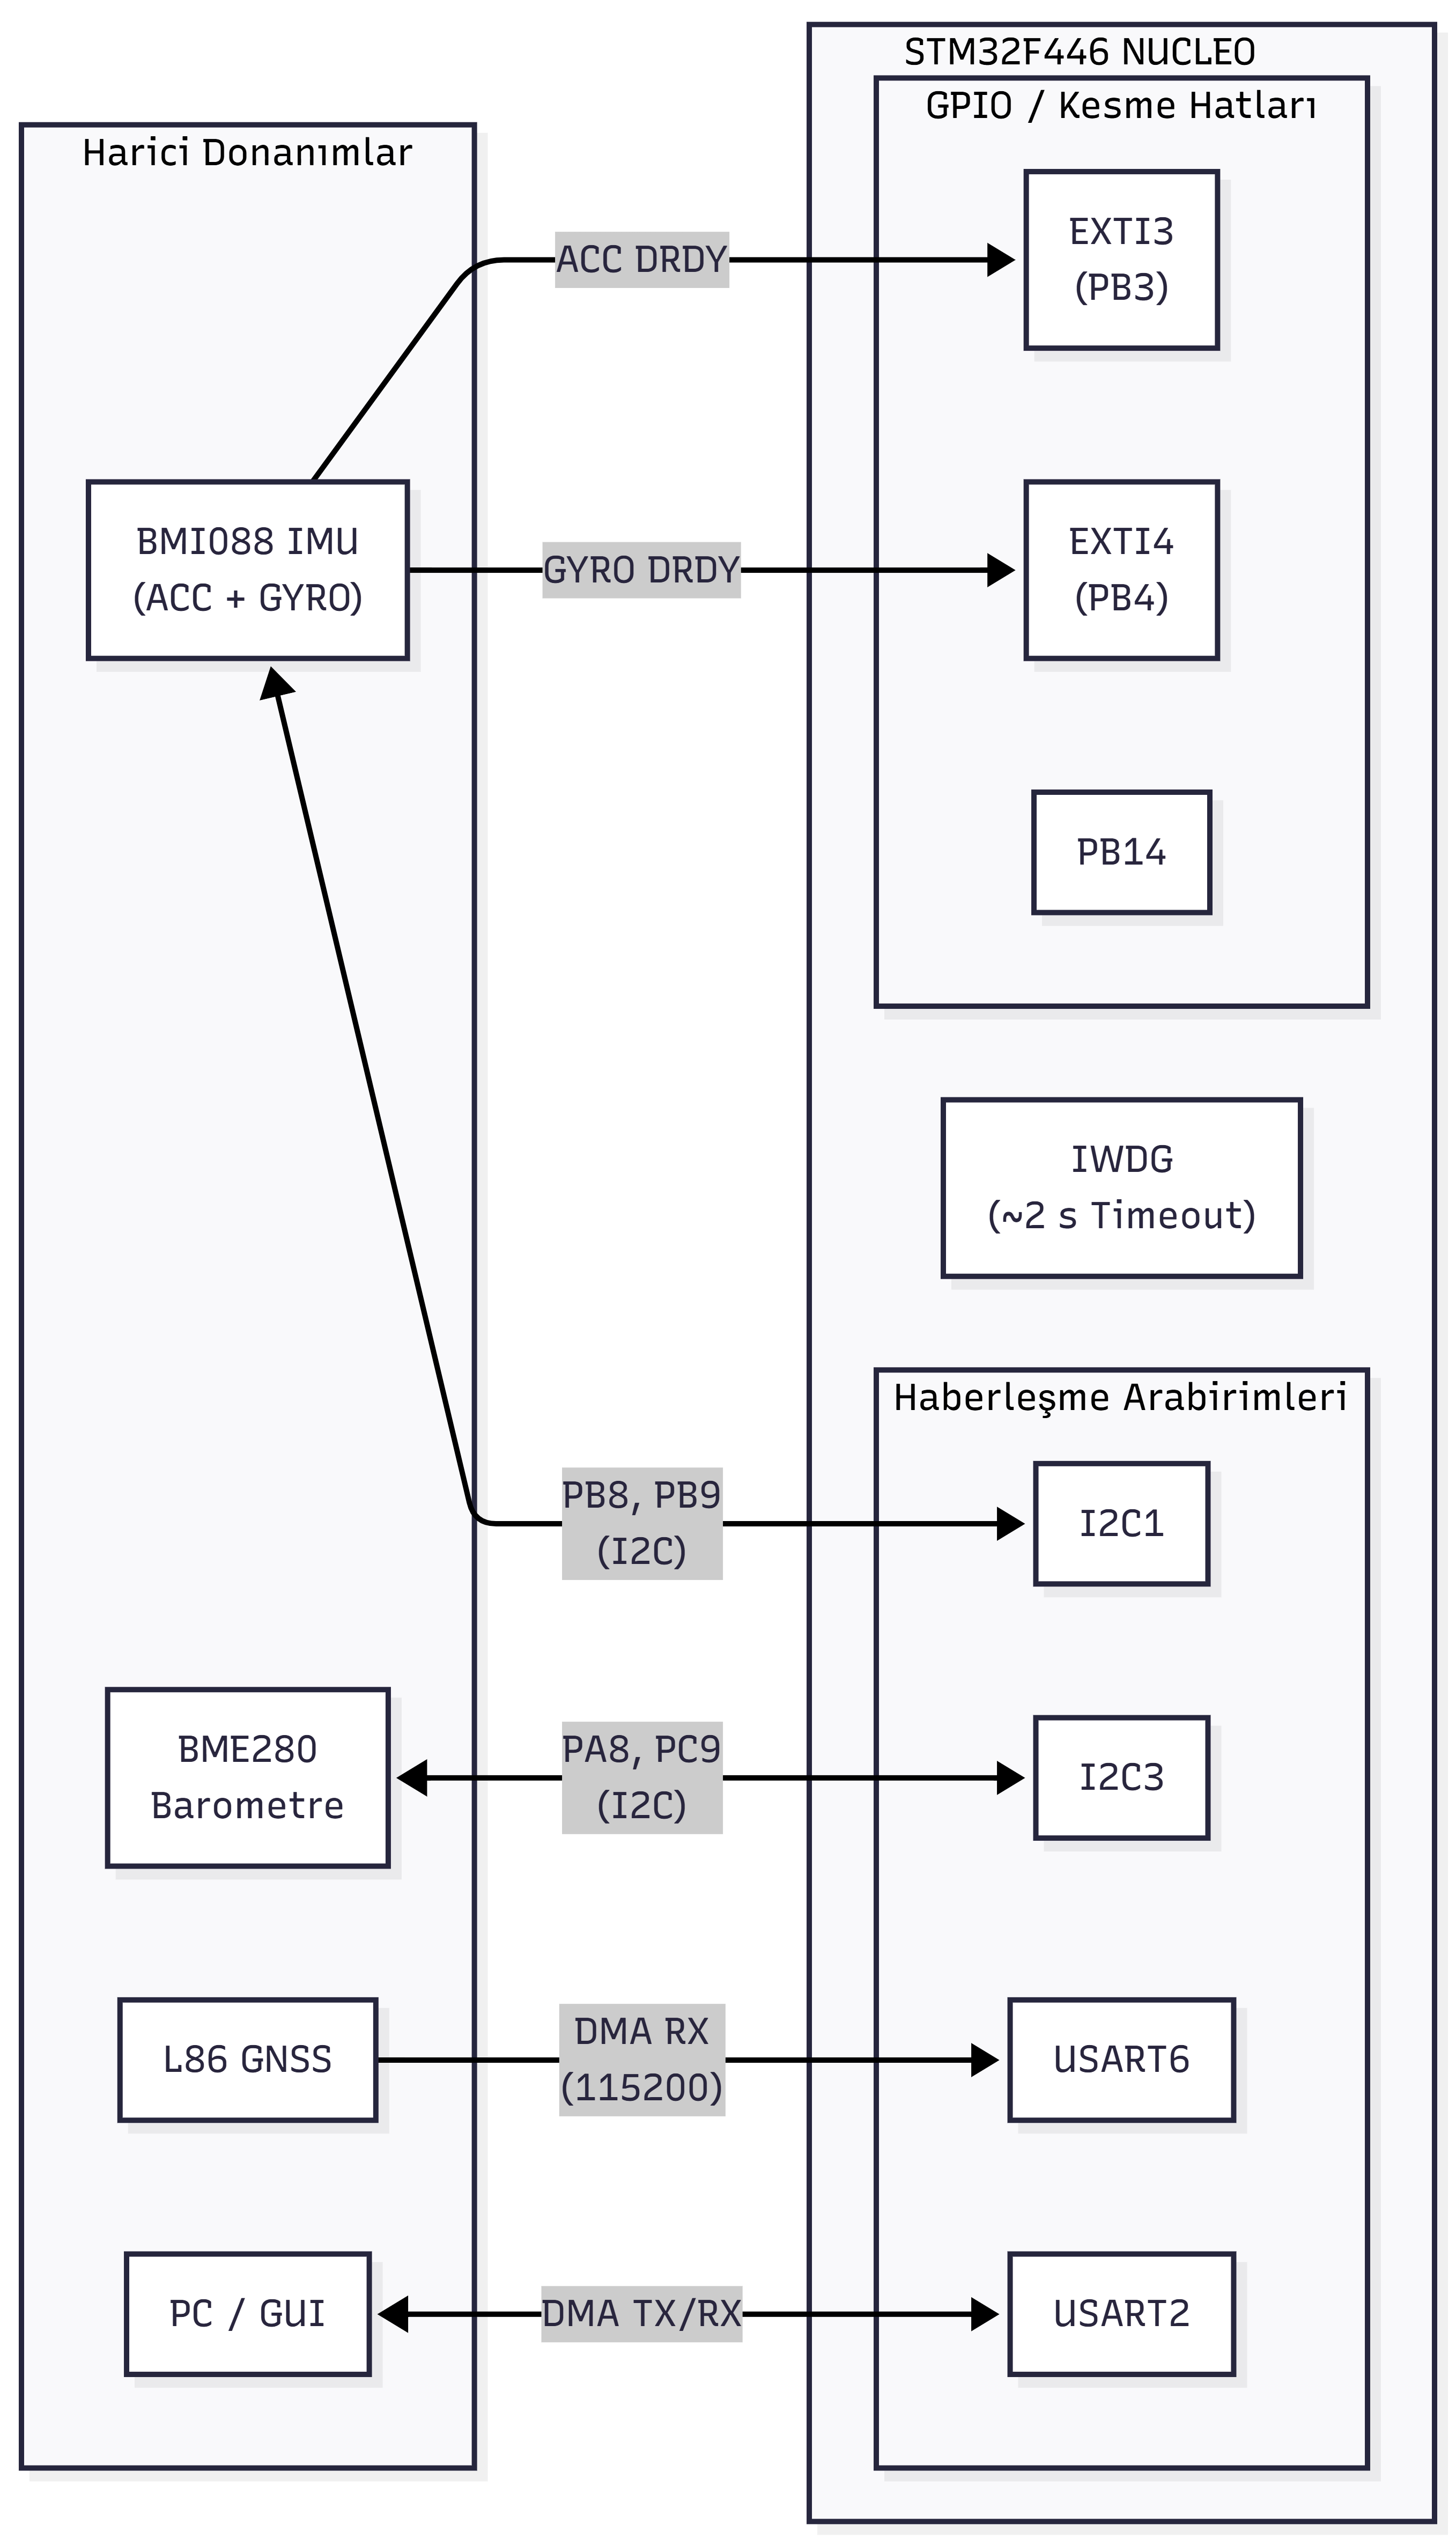
\includegraphics[width=\textwidth]{sekiller/STM32F446DonanımBlokDiyagramı.png}
    \caption{STM32F446 Donanım Blok Diyagramı ve Çevresel Birim Bağlantıları (I2C1$\rightarrow$BMI088, I2C3$\rightarrow$BME280, USART6$\rightarrow$GNSS, USART2$\rightarrow$Telemetri)}
    \label{fig:stm32f446_donanim}
\end{figure}

\subsection{Sensörler ve Ölçüm Altyapısı}
\label{sensorler_altyapisi}
Aviyonik altyapının verimli bir kestirim yapabilmesi için hassas ölçümler gerekmektedir. Sistemin dinamik davranışını okuyan ana unsurlar aşağıda belirtilmiştir:

\begin{itemize}
    \item \textbf{BMI088 (IMU):} Model roket ortamındaki yüksek ivme değişimi ve aşırı sarsıntı koşullarında güvenilir veri okumak için üretilmiş 6 eksenli bir sensördür. $\pm 24g$ ivme ölçüm aralığı ve sarsıntı altında düşük kayma (bias instability) özelliği sergileyen jiroskopu nedeniyle ivme füzyonu için seçilmiştir \cite{bosch_bmi088}. İlgili veri DMA kesmeleri üzerinden işlemciyi engellemeden koşturulur.
    \item \textbf{BME280 (Barometre):} Çevresel basıncı ölçerek Hypsometric algoritması vasıtasıyla mutlak ve bağıl irtifanın hesaplanmasını sağlayan sensördür \cite{bosch_bme280}. Ölçümleme tepki süresinin (response time) IMU sensörlerine kıyasla çok daha yavaş olması sebebiyle (10 Hz civarı), irtifa füzyonunda IMU verileri de algoritmaya katılarak Kalman filtresi destekli çift kaynaklı durum kestirimi kullanılmıştır.
    \item \textbf{L86 (GNSS):} Roketin konum koordinatlarını belirlemek adına saniyede 1 okuma (1 Hz) gerçekleştiren NMEA protokolü tabanlı GPS modülüdür. Baud hızı dinamik geçiş mekanizmaları ile USART üzerinden sürekli aralıklarla durum verisi sağlamaktadır.
\end{itemize}

\clearpage

\section{BÖLÜM: LİTERATÜR TARAMASI}
\label{literatur_taramasi}

Bu bölümde, model roket uçuş bilgisayarı ve yazılım altyapısının inşasında temel alınan bilimsel yöntemler, algoritmik yaklaşımlar ve yazılım mimarilerine yönelik literatür araştırması sunulmaktadır. Geliştirilen sistemin görev yönetimi, durum kestirimi ve uçuş kararlarının teorik altyapısı aşağıdaki alt başlıklarda detaylandırılmıştır.

\subsection{FreeRTOS Mimarisi ve Görev Yönetimi}
\label{freertos_mimarisi_ve_gorev_yonetimi}

Gerçek zamanlı bir görev yürütücüsünde (scheduler), her görev (task) çalışma anında belirli bir duruma sahiptir: \textit{Ready} (Hazır), \textit{Running} (Çalışan), \textit{Blocked} (Bloke) ve \textit{Suspended} (Askıya Alınmış) \cite{freertos_scheduler}. FreeRTOS, \textit{pxReadyTasksLists} isimli listeler üzerinden bu görevleri zamanlar. Yüksek öncelikli bir görev \textit{Ready} durumuna geçtiği an, düşük öncelikli olanı devreden çıkararak işlemciyi ele geçirir (\textit{Preemptive Multitasking}). Bu mekanizma roket yazılımlarında düşük öncelikli telemetri gönderiminin, yüksek öncelikli sensör okuma süreçlerini engellememesini güvence altına alır.

Gömülü sistemlerde Donanımsal Kesme Servis Rutinlerinden (ISR) görevlere veri iletimi, bağlam geçişinin hızını etkileyen kritik bir unsurdur. Çoklu bayrak denetimi (mutex/semaphore) yerine, bekleme süresini minimuma indiren \textit{Task Notification} yapısı kullanılmaktadır. Kesme fonksiyonu içerisinde çağrılan \verb|xTaskNotifyFromISR| ile ilgili göreve sinyal iletilir ve ardından \verb|portYIELD_FROM_ISR| makrosu sayesinde zamanlayıcı işlemciyi doğrudan hazır olan o göreve devreder \cite{freertos_tasks}. Aşağıda geliştirilen sistemde kullanılan DMA tamamlanma kesmesi ve görev bildirim mekanizması örneklendirilmiştir:

\begin{figure}[H]
    \centering
    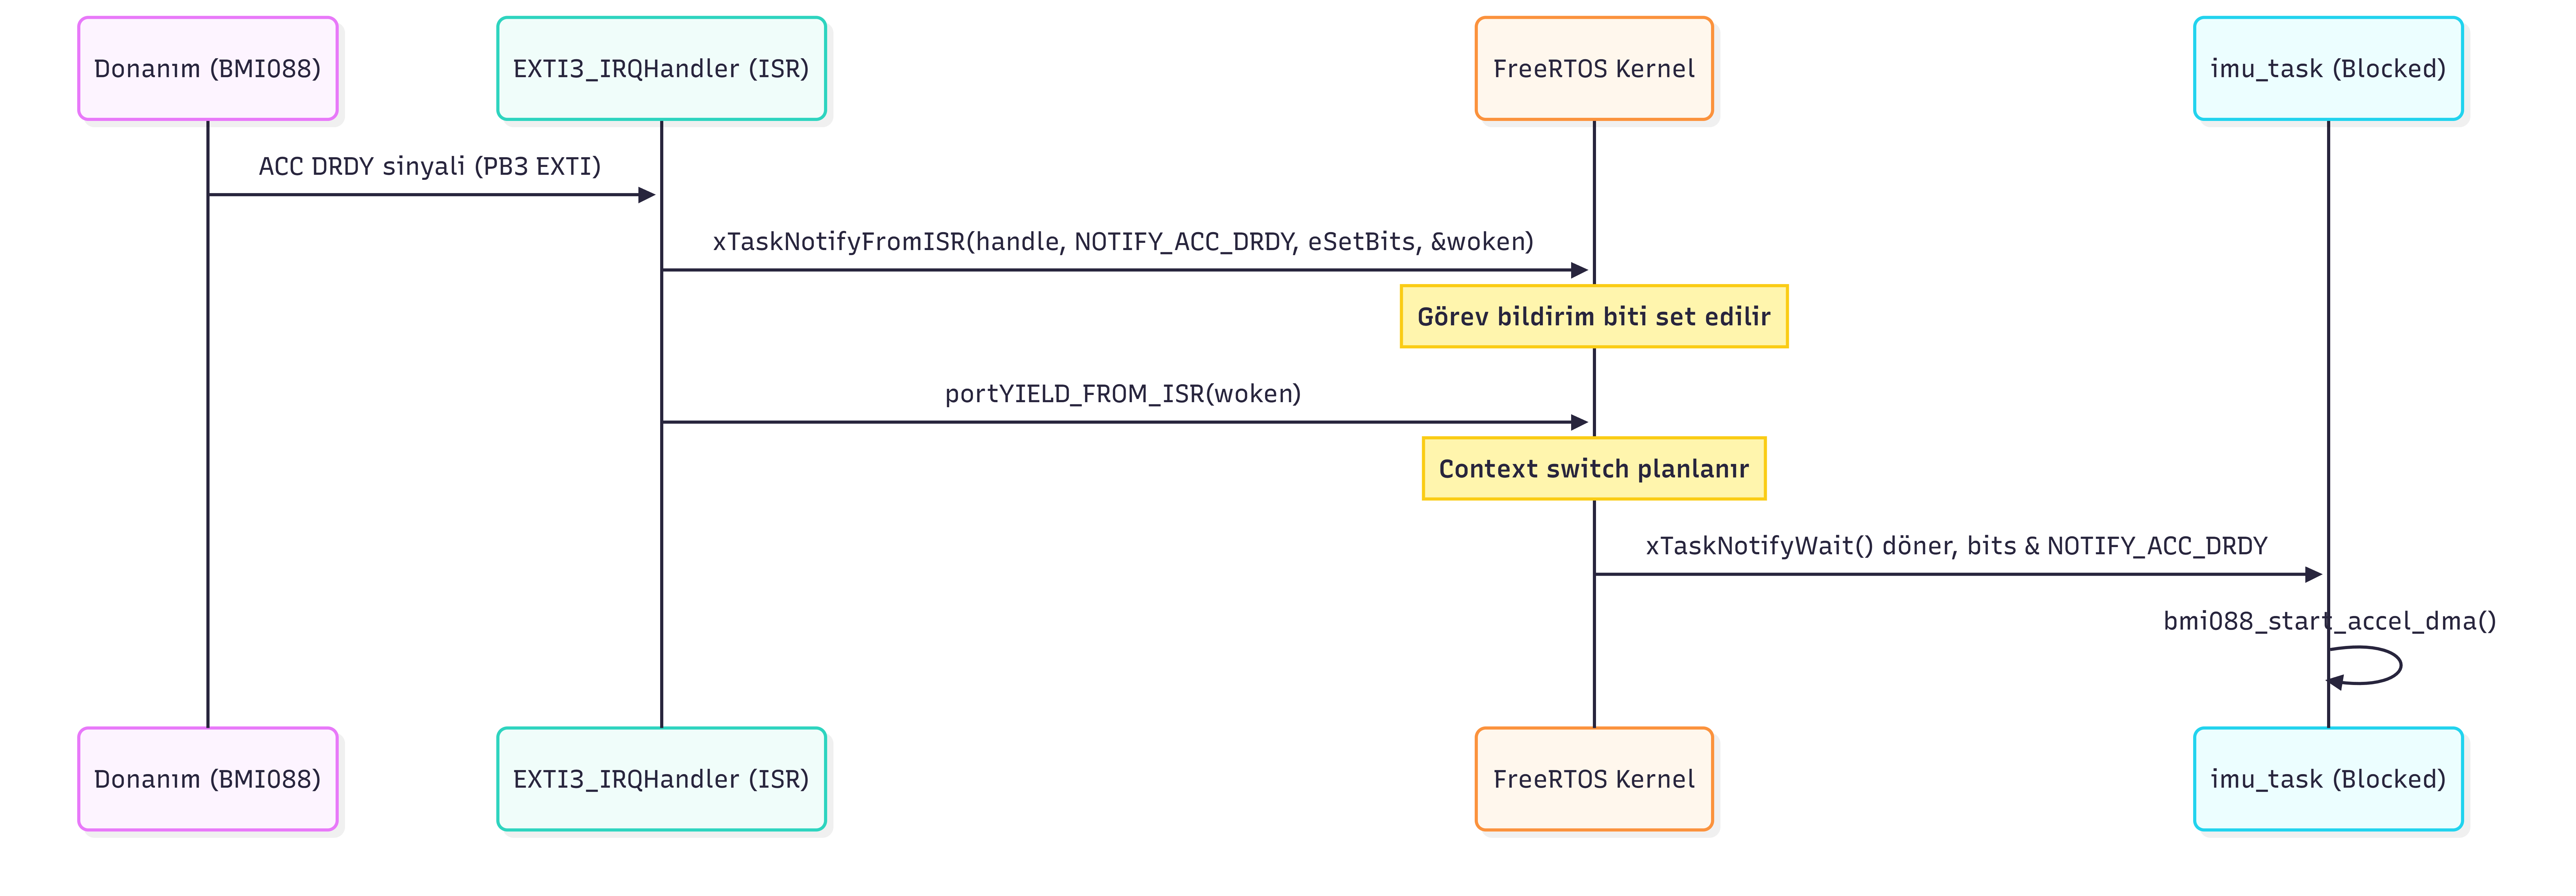
\includegraphics[width=0.8\textwidth]{sekiller/TaskNotificationKalıbı.png}
    \caption{ISR ve Task Arasında Task Notification Sinyalleşme Mimarisi}
    \label{fig:task_notification}
\end{figure}

\begin{lstlisting}[language=C, caption={Kesme Servis Rutini (ISR) İçerisinde Task Notification Kullanımı (\texttt{imu\_task.c})}]
void HAL_I2C_MemRxCpltCallback(I2C_HandleTypeDef *hi2c)
{
    if (hi2c->Instance != I2C1 || s_handle == NULL) return;

    BaseType_t woken = pdFALSE;
    xTaskNotifyFromISR(s_handle, NOTIFY_DMA_DONE, eSetBits, &woken);
    portYIELD_FROM_ISR(woken); // Eger imu_task hazir ise aninda baglam degistir
}
\end{lstlisting}

Görevler arası durum paylaşımı (Snapshot mekanizması) için Derinliği 1 (\textit{depth=1}) olan kuyruklar (Queue mailbox pattern) tercih edilmiştir. \verb|xQueueOverwrite| kullanılarak eski veri silinip sürekli yeni uçuş verisi yazılır (Producer) ve diğer görevler tarafından eksiltme olmadan kopyası alınabilmesi için \verb|xQueuePeek| fonksiyonu kullanılır (Consumer) \cite{freertos_queue}. Kuyruk derinliğinin 1 olması, bellekte gereksiz tamponlama (buffering) yapılmasını engelleyerek her görevin son uçuş durumuna erişmesini garanti etmektedir.

\begin{figure}[H]
    \centering
    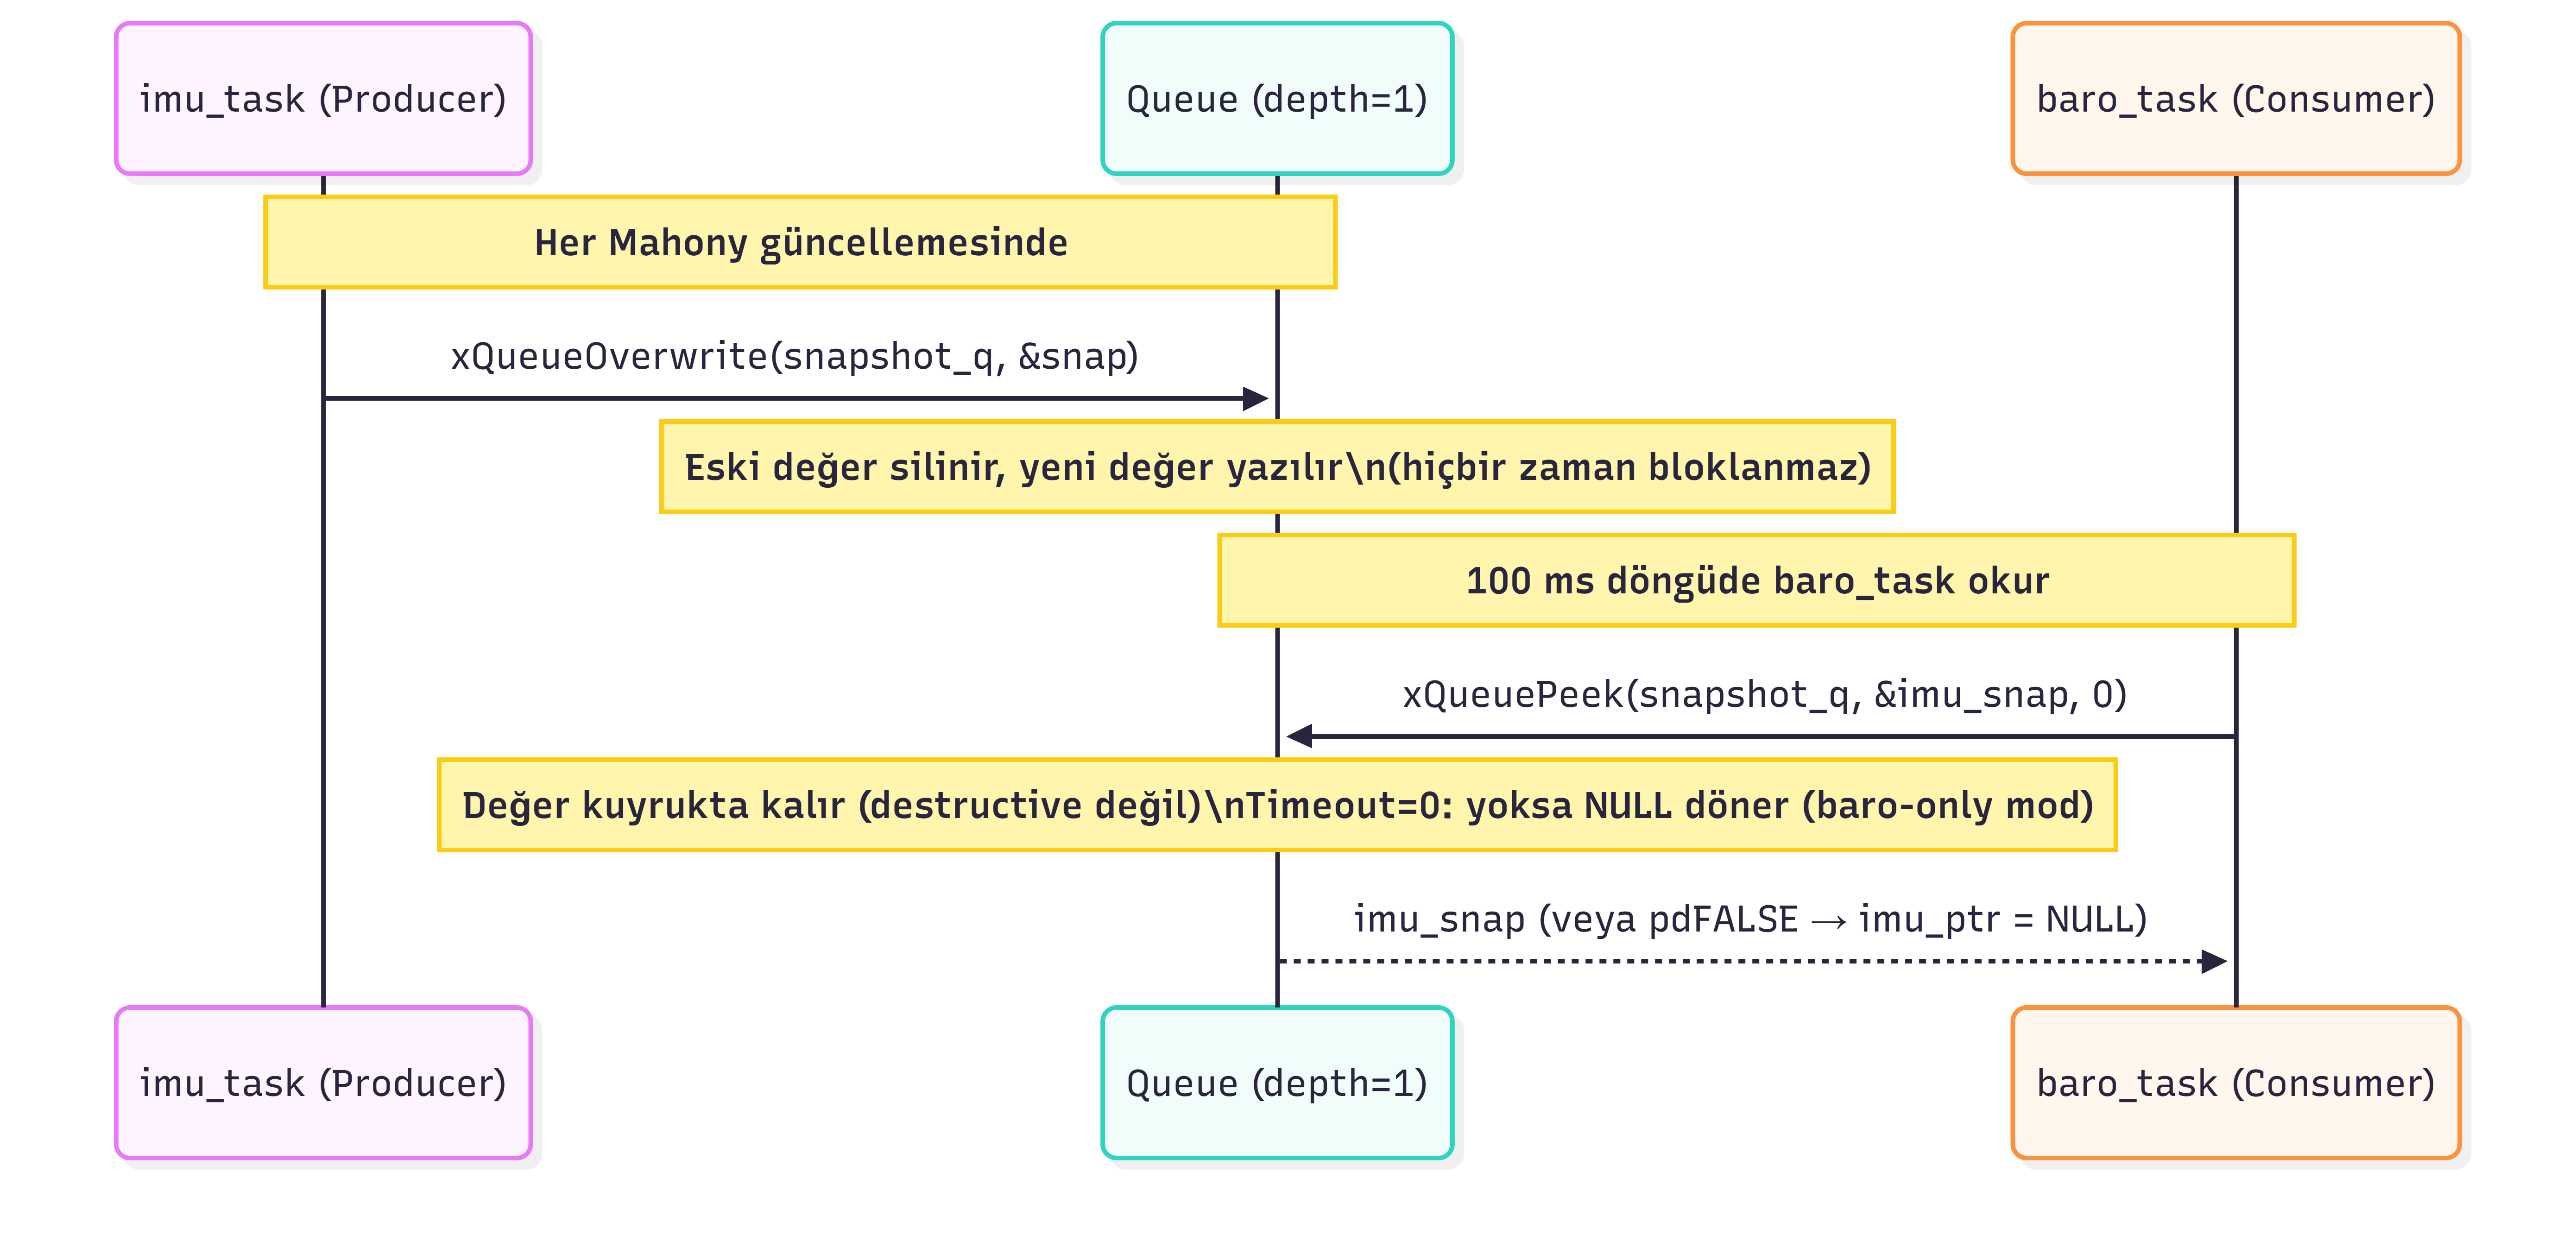
\includegraphics[width=0.8\textwidth]{sekiller/TaskSnapshotQueueKalıbı.png}
    \caption{Görevler Arası Derinliği 1 Olan Kuyruk (Snapshot Queue) Veri Paylaşım Kalıbı}
    \label{fig:task_snapshot}
\end{figure}

\subsection{Sensör Füzyonu Yöntemleri (Mahony, Kalman)}
\label{sensor_fuzyonu_yontemleri}

Roketlerin fırlatma anı esnasında maruz kaldığı şiddetli titreşimler ve motor ivmesi, salt ivmeölçer verisini son derece gürültülü hale getirir. Diğer yandan jiroskoplar gürültüden daha az etkilense de, zamanla küçük sapmaların matematiksel bütünleştirilmesi dolayısıyla kayma hatası (drift) üretir. Bu nedenle füzyon işlemi zorunludur \cite{stanford_imu_notes}. Geleneksel \textit{Tamamlayıcı Filtre} (Complementary Filter) yaklaşımı, jiroskopun kısa dönem kararlılığı ile ivmeölçerin uzun dönem doğruluğunu;

\begin{equation}
\theta_{t} = \alpha \left( \theta_{t-1} + \omega \Delta t \right) + (1 - \alpha)\theta_{acc}
\end{equation}

denklemiyle birleştirir \cite{ahrs_doc}, fakat bu fırlatma esnasındaki eksen kaymalarında yetersiz kalmaktadır. Projede Euler açı açmazını (Gimbal Lock) ortadan kaldıran ve oransal-integral (PI) hata geri beslemesi mantığıyla çalışan \textbf{Mahony Filtresi} tercih edilmiştir \cite{ahrs_mahony_doc, madgwick2011estimation}. Burada yerçekimi tahmin vektörü $\hat{\mathbf{g}}$ ile normalize edilen tahmini ivme vektörü $\mathbf{a}_{norm}$ arasındaki hata ($e$) Vektörel Çarpım yoluyla belirlenir:

\begin{equation}
\mathbf{e} = \hat{\mathbf{g}} \times \mathbf{a}_{norm}
\end{equation}

Bu hata hesaplandıktan sonra, Quaternion ($q$) entegrasyonu; jiroskop ölçümleri, jiroskop sapmasını dengeleyen entegrasyon terimi ($\mathbf{b}$) ve hata ($e$) vektörünün katılması ile sürekli yenilenmektedir:

\begin{equation}
\dot{q} = \frac{1}{2} q \otimes \left( \omega_{gyro} - \mathbf{b} + K_p \mathbf{e} + K_i \int \mathbf{e} \, dt \right)
\end{equation}

İrtifa Füzyonu aşamasında ise sistemdeki \textit{Baro (BME280)} ile \textit{IMU (Z ekseni)} entegrasyonu \textbf{Kalman Filtresi} aracılığıyla gerçekleştirilmektedir \cite{welch1995introduction}. Kalman filtresinde durum vektörü $\hat{x}_k = [ \text{İrtifa}, \text{Hız}, \text{İvme\_Bias} ]^T$ şeklinde konumlandırılmıştır. Sabit ivme kullanılarak varsayılan durum geçiş matrisi ($F$):

\begin{equation}
\hat{x}_{k|k-1} = F \hat{x}_{k-1|k-1} + B \cdot u_{k}  \quad , \quad
P_{k|k-1} = F P_{k-1|k-1} F^T + Q
\end{equation}

Denklemlerde belirtilen $Q$ süreç (process) gürültüsünü, hesaplanan barometre verilerindeki gürültü kovaryans matrisi $R$ ise ölçüm gürültüsünü ifade eder. İkinci adımda kazanç ($K$) oluşturulur ve gözlem matrisi ($H$) ile ölçülen veri kullanılarak yapı güncellenir:

\begin{equation}
K_k = P_{k|k-1} H^T (H P_{k|k-1} H^T + R)^{-1}
\end{equation}

\begin{equation}
\hat{x}_{k|k} = \hat{x}_{k|k-1} + K_k (z_k - H \hat{x}_{k|k-1})
\end{equation}

\subsection{Uçuş Durum Makinesi Yaklaşımları}
\label{ucus_durum_makinesi_yaklasimlari}

Bir roketin kalkış öncesinden yere inene değin geçen fazları algoritmik bir biçimde idare edebilmek için Durum Makinesi (Finite State Machine - FSM) konseptleri öne çıkmaktadır. Literatürde güvenilirliği sağlamak amacıyla FSM mimarileri kullanılmaktadır; çünkü bu tasarımlar \textit{if-else} spagetti kod karmaşasını önler, olaylar arası tetikleyicilerin izlenebilirliğini (traceability) artırır ve roket kurtarma fırlatmalarının yanlış fazlarda gerçekleşmesini izole eder. 

Model roket projelerinde literatür çerçevesinde tanımlanmış ve geliştirilmiş temel operasyon fazları: IDLE (Hazır Bekleme), BOOST (Kalkış İvmelenmesi), COAST (Serbest Uçuş/Süzülme), APOGEE (Tepe Noktası - Drogue Paraşütü), DROGUE\_DESCENT (1. Aşama İniş), MAIN\_DESCENT (2. Aşama Ana Paraşüt İnisi) ve LANDED (Yere İniş) adımlarından oluşmaktadır. Apogee (Tepe Noktası) tespit algoritmalarında yaşanabilecek yanılmaların önüne geçmek adına çoklu tepe noktası mekanizmaları tanımlanmıştır; \textit{hız bazlı apogee} (Kalman filtresinden gelen düşey hız vektörünün 0'ın altına inmesi) ile yönelime duyarlı \textit{tilt bazlı apogee} (Mahony tahmini Pitch açısının (theta) 70$^\circ$'nin üzerine çıkması). Bu iki şarttan birinin tetiklenmesiyle sistem duruma otomatik olarak geçiş yapmaktadır.

\clearpage